\chapter{Modelado de Solución}
Como se ha mencionado en el capitulo de situación actual, el problema principal surge por la no utilización
de métodos que permitan validar los documentos digitales, emitidos por la Secretaría de Extensión de la \gls{unam}, 
en este apartado se explica como abordar la solución a este problema.

\section{Propuesta de solución}

En cuestiones generales para solucionar los problemas se propone realizar un sistema que permita a la 
Secretaría de Extensión de la \glsfirst{unam} :

\begin{enumerate}
    \item Dar validez a un documento por tiempo determinado y gestionar sus estados.
    \item Que entidades externas puedan validar la integridad de documentos digitales emitido por la Universidad.
    \item Permitir acceso a todo público el uso del sistema para la validación.
    \item Proteger la privacidad de los datos que pertenecen a los documentos.
\end{enumerate}

Los items descritos, se pueden lograr con la utilización de la tecnología Blockchain, 
otorgando inmutabilidad a los datos almacenados y que sean accesibles a todo público.
En cuanto a protección de la privacidad es necesario utilizar, algún método criptográfico 
para que los datos sean leidos, usados solo por las partes autorizadas.
Y por último para que las entidades o cualquier individuo pueda validar que el documento digital, es el mismo
que emitió la \gls{unam} se debería crear un relación con los documentos digitales emitidos por ella misma. 

\subsection{Procesos para la construcción del sistema}
Serán necesarios para el diseño, modelado y desarrollo de la solución definir las herramientas a utilizar,
y los pasos.
\begin{enumerate}
    \item Definición de métodos, tecnologías y herramientas a utilizar.
    \item Diseño de la solución.
    \item Desarrollo del diseño propuesto.
    \item Pruebas y validaciones del funcionamiento.
\end{enumerate}


\section{Descripción del modelo}

Se pretende realizar una propuesta de sistema, que permita al usuario consultar la validez  de sus documentos digitales   por la entidad que la emitió
  y cuando se ha publicado.
Que permita a los gestores de la organizaciones subir  nuevos documentos o algún identificador del documento para comprobar
de manera inequívoca si fue emitido por ellos, también mostrar datos relacionados, como ser en que evento se ha generado 
el documento o en que institución u organización.
Con esta propuesta de sistema, cubriría los aspectos mencionados en cuanto a las necesidades de brindar una medio por el cual
se pueda verificar que los documentos de las actividades desarrolladas por la  
  Secretaría de Extensión de la \gls{fce} puedan ser verificados y dar validez que el contenido del mismo no fue adulterado, modificado o cambiado.


\subsection{ Análisis de Tecnologías}
Para poder realizar la propuesta de sistema, hay que determinar que tecnologías y alternativas son necesarias para llevarla a cabo.
Existen distintos tipos de modelos para validar los certificados con la  Blockchain como lo son  s visto en la  página \pageref{sssec:blockcerts} o OpenCerts 
descrito en la  página \pageref{sssec:opencerts}.

s es un estándar abierto  que permite  almacenar y verificar documentos en la Blockchain,
generar el hash a partir de un certificado o documento y lo almacenan en una transacción, de la red de Bitcoin o Etherum o en cualquier otra.
El estándar es muy util y cuenta con una aplicación movil para poder verificar los documentos digitales, 
donde los usuarios pueden obtener una cuenta propia. Su funcionamiento esta descrito en el propio sitio web \footnote{\url{https://www.blockcerts.org/guide/quick-start.html}}.

\begin{figure}[hbt!]
  \centering
  {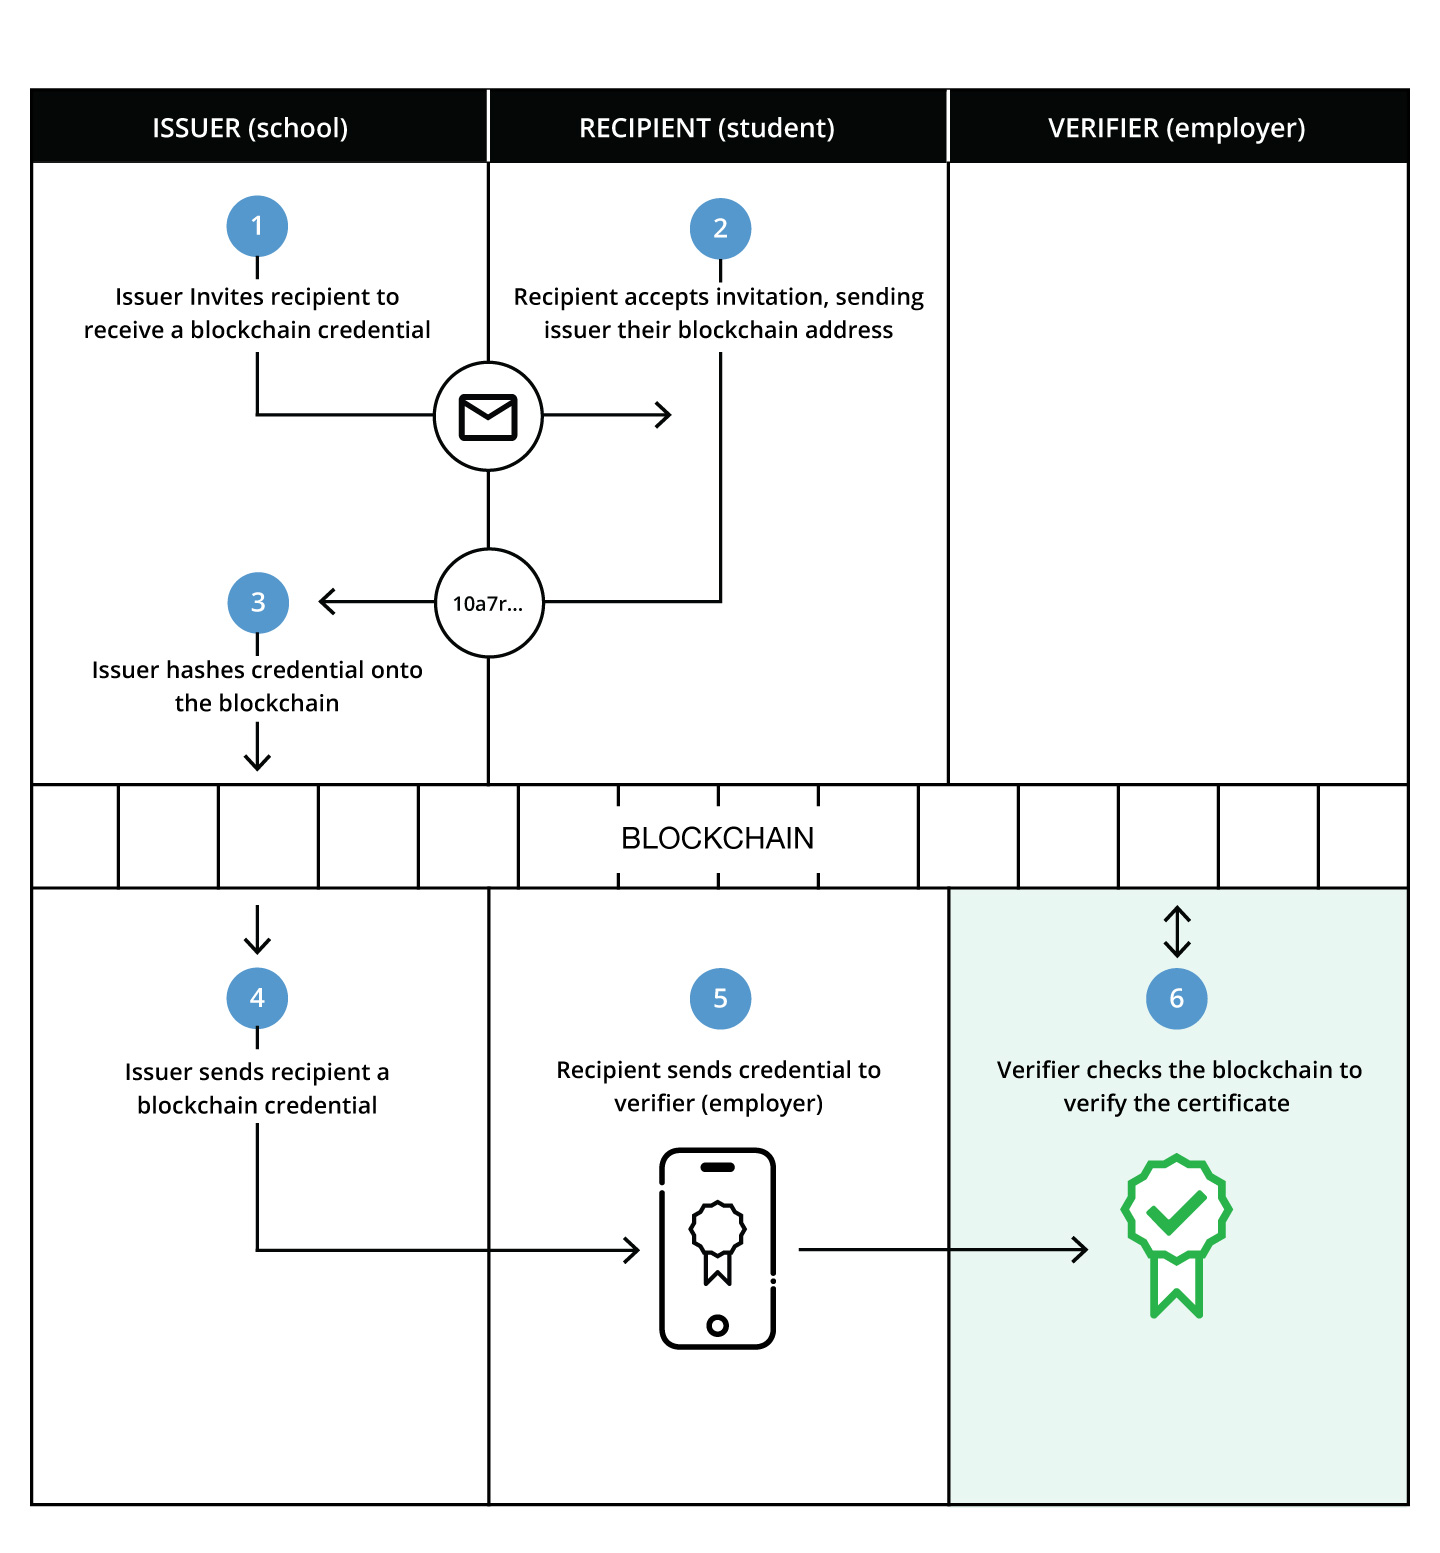
\includegraphics[scale=0.3]{blockcerts_how_it_works.jpg}}
  \caption{Imagen extraída de la página oficial de s}
  \label{img:blockcerts_how_it_works}
\end{figure}


En el paso 1 el emisor o institución invita a un usuario que le envié su dirección de cuenta o su clave pública creada 
descargando la aplicaciones movil que provee s. En el paso 2 el usuario enviá al emisor su clave pública,
en el paso 3 y 4 el emisor crea el hash a partir del certificado y lo almacena en la  Blockchain para luego enviar un archivo json, que contiene
la información sobre el documento al estudiante o dueño del certificado, el en el paso 5 puede enviar este documento a cualquier empresa o individuo que dese.
y por último en el paso 6 el que contiene el archivo puede verificarlo en la  página web de blockcerts. Este es el flujo básico que también se 
puede visualizar en  la figura \ref{img:blockcerts_how_it_works}   para comprobar que
un certificado se encuentra almacenado en la  Blockchain y es validado por un instituto.\cite[]{blockcerts_introduction_nodate}

% Este estándar es muy completo y permite a los usuarios gestionar sus propios certificados, pero lo que se busca en la investigación, 
% es desarrollar una propuesta de sistema donde un usuario puede abstraer el concepto de  Blockchain sin controlar una cuenta, enfoncadonce solamente en mantener guardados
% sus certificados.


Otra tecnología es OpenCerts, \footnote{https://www.opencerts.io/} funciona, generando 
un código único a partir del certificado e información extra considerada como necesaria para validar el documento en el futuro, luego se crea un archivo con extensión  “.opencerts ”;
el archivo se sube a la  página de opencerts y compara el contenido con el almacenado en la  Blockchain para verificar si a existido el certificado en cuestión.
Para dar de alta los certificados usa smart contract donde también crean los métodos para emitir o revocar un documento.

\begin{figure}[hbt!]
  \centering
  {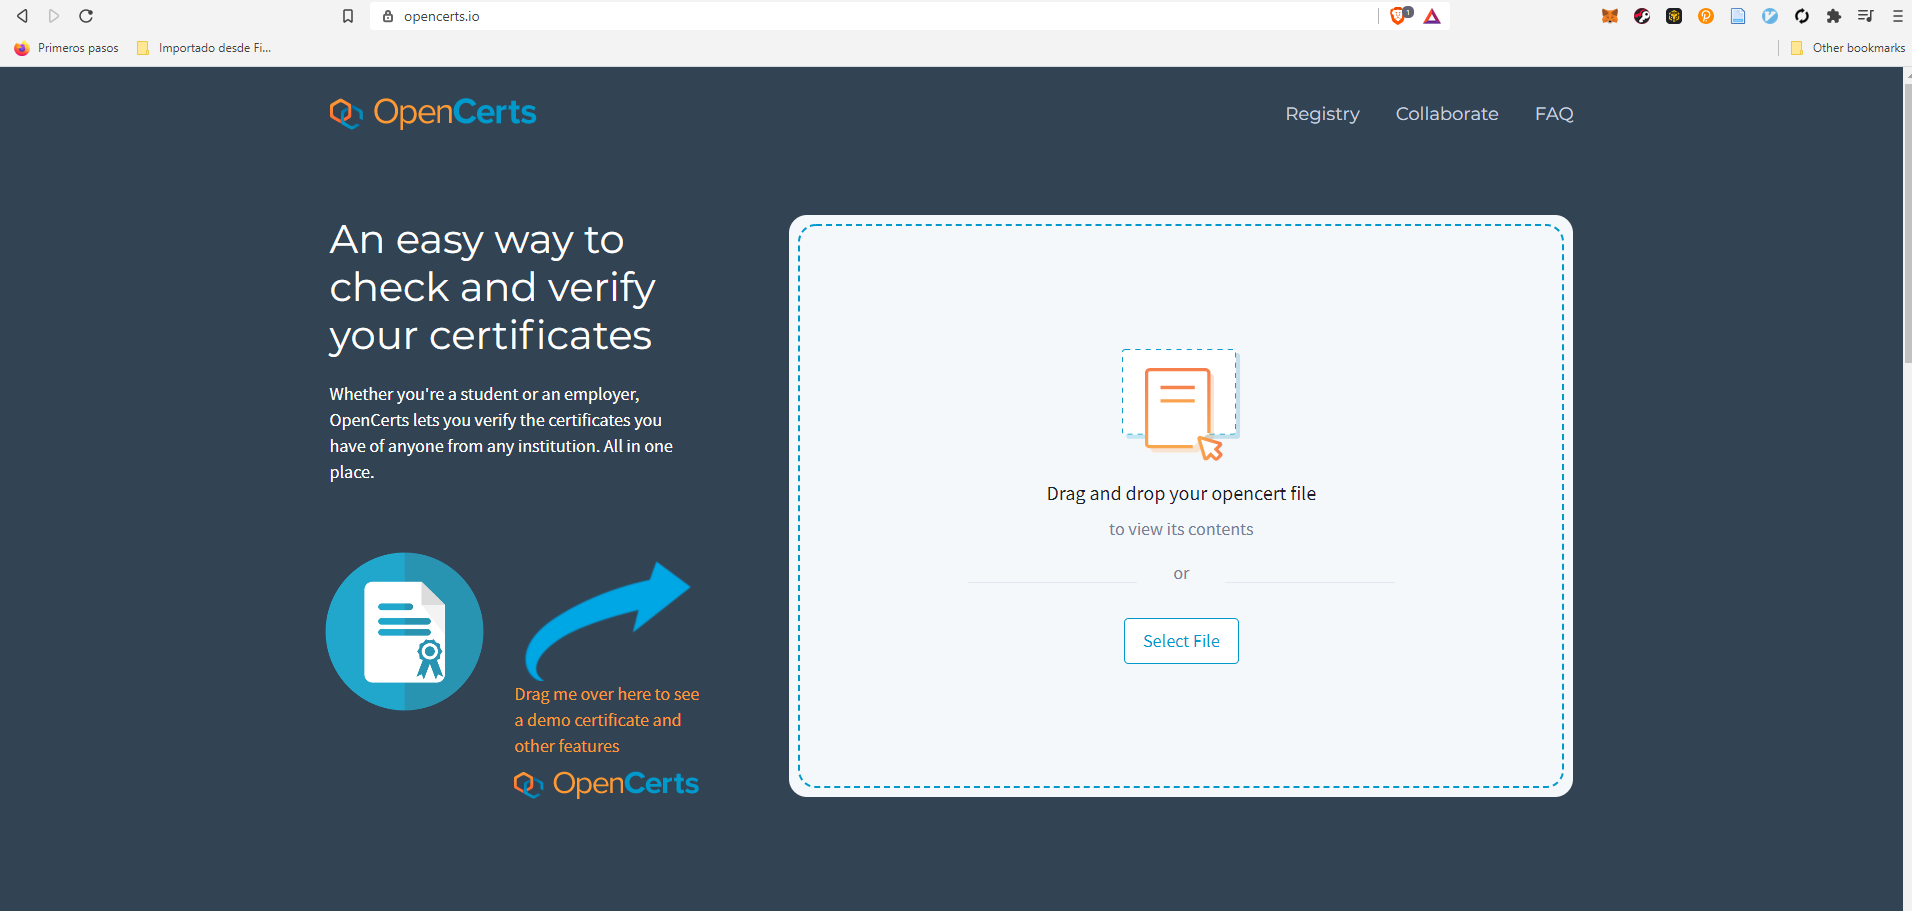
\includegraphics[scale=0.3]{OpenCerts_Home.png}}
  \caption{Pagina Web de OpenCerts}
  \label{img:opencerts_home}
\end{figure}

En la imagen \ref{img:opencerts_home} se puede observar lo sencillo que es verificar un documento, simplemente arrastra su  archivo “nombre-archivo.opencerts”
y se buscará en la  Blockchain si realmente fue emitido por alguna entidad.
OpenCerts utiliza los smart contract en la  Blockchain de Etherum, también utilizo tecnologías como Ract.js, Metamask, Web3.js, entre otros. Permitiendole desarrollar
un sistema de certificados totalmente descentralizado. \cite[]{opencerts_gestion_nodate}


Por último también se encuentra la \glsfirst{bfa} la cual es una  Blockchain que utiliza el protocolo de consenso llamado como Proof of Authority explicado en la sección 
\ref{sec:poa}, en el sitio web cuenta con una herramienta llamada sello de tiempo 2.0, que permite verificar cuando se ha sellado un archivo y en que bloque,
permitiendo confirmar que desde esa fecha el archivo en cuestión no ha sufrido modificaciones. Utiliza el mismo método que las anteriores tecnología, 
crear un hash a partir de un archivo y almacena el hash en la Blockchain.

En resumen todas estas tecnologías, permiten demostrar que una secuencia de bits o cualquier tipo de archivo (pudiendo ser
 un documento o certificado) se mantuvo inalterable a partir del dia que se ha almacenado en la  Blockchain su hash o identificador único. Algunas de ellas 
cuentan con un flujo y trabajo mas elaborado, pero al fin todas cumplen con el objetivo de asegurar a los interesados si existió algún cambio en datos
del documento o archivo en cuestión. 
Luego de analizar el funcionamiento de estas, se pretende realizar una propuesta de sistema, que permita a una institución principalmente 
a la \gls{fce} emitir sus certificados y a los participantes de los eventos  demostrar que sus 
certificados o documentos digitales son totalmente auténticos y correspondiente  a su persona. 

\subsection{ Análisis de Herramientas}
Existen diferentes herramientas para elaborar un sistema que necesita comunicarse con una red de peer to peer y leer o escribir en la Blockchain,
Primero habría que definir como se almacenaría la información en al Blockchain, si almacenarlo en uan transacción de cualquier  Blockchain como lo hacer
s o realizar una lógica y almacenarla en una  Blockchain que soporte contratos inteligentes;
La ventaja de los smart contract es que permite almacenar información especifica como ser el nombre de una institución, sus participantes o
cualquier información que se desee en una sola transacción o invocación a un método del smart contract, mientras que el primer método se necesitaría 
almacenar diferentes datos en diferentes transacciones, o realizar un hash que representará que un documento sigue inalterable.
Por conveniencia de la investigación almacenar datos en los smart contract, permitiría obtener información directamente de 
la  Blockchain sin uso del hash mediante la recuperación del dato literalmente, como ser el nombre de la institución y podría ser visualizada por cualquier 
individuo que consulte el smart contract, esta diferencia da lugar a la creación de aplicaciones, por la 
conveniencia de almacenar datos que pueden ser recuperados y leidos permitiría generar un nivel de seguridad que en el caso que el  emisor
desaparezca, se podrá obtener la información de quien era la institución, en comparación
con el estándar de s que permite hacer lo mismo, pero se necesitaría el archivo que almacena toda la información del emisor.\cite[]{blockcerts_introduction_nodate,opencerts_gestion_nodate}
A partir de este punto se enumeran las diferentes herramientas necesaria para el desarrollo de un sistema de validación de certificados usando Blockchain.

\subsubsection{Programación en Blockchain}

Habría que decidir en que  Blockchain se trabajaría, porque los smart contract se escriben en un lenguaje específico,
en el caso de Etherum es Solidity, pero existen un gran numero de  Blockchain que utilizan la misma estructura de Etherum para generar 
su propia  Blockchain con algunas diferencias, pero en cuanto al lenguaje de programación  para el desarrollo de los smart contract 
es el mismo. En este caso se utilizaría Solidity, donde se define como un lenguaje orientados a objetos influenciado  por
C++,Python y JavaScript. \cite[]{dannen_introducing_2017,ethereum_solidity_nodate}

\subsubsection{Comunicación con Blockchain}
Es necesario un metodo o herramienta para comunicar las transacciones que se deben realizarse 
en la Blockchain, para ello se precisa de una Wallet o Billetera que permita enviar las transacciones 
y comunicarse con los smart contract, en este caso existen diferentes wallet, pero una de las mas usada
es Metamask \footnote{\url{https://metamask.io/}}, permite gestionar las cuentas de los usuarios de manera local, conectarse con diferentes Blockchain, 
recibir y enviar dinero e interactuar con los Smart Contract.
Es un puente entre una Aplicación y la Blockchain, usada por desarrolladores. \cite[]{dannen_introducing_2017,metamask_introduction_2021}

 








Inicialmente 
(Escribir todo lo que voy a usar, desde tecnologías, como se planteara el problema, metodos etc.)
(hacer comparaciones econ metodos y elejir cuales se van a usar, por ejemplo que tipo de hash se va a utilizar
en este capitulo conta algunos metodos del hash y cuales vas a usar.)

(smart contract se va usar, que  Blockchain se va  usar de prueba, en cual se va implementar )







